\documentclass[12pt]{article}
\usepackage[]{cite}   % remove to use brackets instead of superscripts in citations
\usepackage{graphicx}
\usepackage{fancyhdr}
\usepackage{xcolor}
\usepackage{indentfirst}
\usepackage[a4paper, portrait, margin=1in]{geometry}
\usepackage{lastpage}
\usepackage{float}
\usepackage{tabularx}
\pagestyle{fancy}
\fancyhf{}
\fancyhead[L]{Vupiter}
\fancyhead[R]{Project Proposal}
\rfoot{Page \thepage \hspace{1pt} of \pageref*{LastPage}}
\pagenumbering{arabic}
\newcolumntype{L}{>{\centering\arraybackslash}m{3cm}}
\usepackage[pdftex,bookmarks,pdfpagemode=UseOutlines,
    pdfauthor={Vupiter Team},
    pdftitle={Project Proposal},colorlinks=true, linkcolor=blue]{hyperref}
% removed colorlinks after bookmarks

\newcommand{\code}[1]{\texttt{\smaller #1}}

\setlength\parindent{5ex}
\setlength\parskip{2ex}
\newcommand\xrowht[2][0]{\addstackgap[.5\dimexpr#2\relax]{\vphantom{#1}}}
\newcommand{\fig}[1]{\centerline{\includegraphics{#1}}}

\DeclareGraphicsExtensions{.pdf, .jpg, .png}
%\setkeys{Gin}{width=0.85\textwidth}
\begin{document}
\begin{titlepage}
    \begin{center}
        \vspace*{1cm}
            
        \Huge
        \textbf{Vupiter DC Power Supply}
            
        \vspace{0.5cm}
        \large
        Date: \today
            
        \vspace{2.25cm}

        \textbf{Senior Design Mid-term Report}
        
        \vspace{2.25cm}

        \textbf{Team Members:}\\
        Chase Flatau\\
        Alex Jones\\
        Rice Shelley\\
        Al Spies\\
        \textbf{Faculty Advisors:}\\
        Doctor Robert Nelms\\
        Doctor Thadeus Roppel
        \vfill
            
            
        \vspace{0.8cm}
            
        
\includegraphics[width=0.4\textwidth]{university}
            
        \Large

        \textbf{Auburn University}\\
        Department of Electrical and Computer Engineering\\

            
    \end{center}
\end{titlepage}

\tableofcontents
\pagebreak

\section{Introduction - Rice Shelley}
Vupiter DC power supply has three independent isolated channels each with an output of 0 - 30V at 5A and a resolution of 10ma / 10mv. The power supply features a physical front panel as well as a desktop computer interface. The physical front panel allows for normal lab operation while the virtual front panel can be used for test automation. The virtual front panel will comply with industry standards for interfacing programmable instruments so that preexisitng software may be used with the Vupiter power supply. Vupiter is entirely open source to allow for easy modifications and tailored functionality. Vupiters comparatively low cost will provide accessibility for hobbyists and makers. Multi-channel power supplies are typically priced in the \$300 plus range. Vupiter will provide a comparatively affordable option in the \$100 range with similar functionality. The price of the supply can be lowered by allowing hobbyist to purchase the PCB’s and parts to assemble the power supply themselves.

\section{Topology - Chase Flatau}
The Vupiter project is a three-channel power supply; therefore, there are three separate lines for each channel. Each channel will be fed from a single Power Factor Correction board before splitting. This is followed by a switched power mode board, a linear power board, and finally a human interface. The first stage is the power supply to our power supply which will be a standard wall outlet which leads into the PFC stage. The PFC will take the wall output, 85-265 VAC, and convert it to 400 VDC. Only one of these are needed for the three isolated channels. This in turn leads into the three switched mode boards. Each of these boards control their individual channel and can work independently of the other two. Each one will take the 400 VDC and output 36-6 VDC at a max of 5.5 A. There is a built in 6 VDC and 0.5 A built in for the linear stage to use for control.\\

The next stage is the linear power boards. These boards control the final output of each channel. This is accomplished through op-amps and a microchip controlling BJTs. The maximum output for a single channel is 36 VDC at 5 A. All of this is controlled by a human interface, either through the respective front panel controls or a USB connection to a computer. Each channel will have its own OLED screen to display the current settings and its own set of push knobs to control voltage and current. The power supply can also be controlled through a provided GUI or any program that the user may design and send over SCPI. Due to the open sources used, the user has a large degree of freedom to change what they want to better fit what they need.\\

\begin{figure}[H]
    \centering
    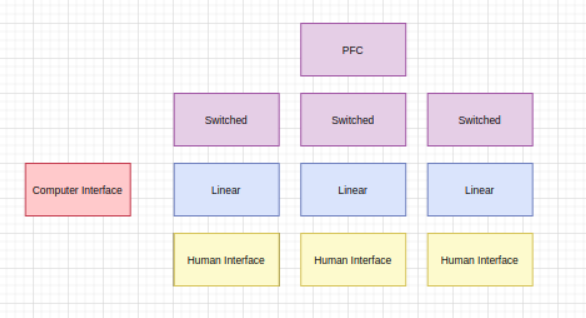
\includegraphics[width=0.8\textwidth]{chase1}
    \caption{Switching Section}
    \label{fig:chase1}
\end{figure}

\section{Linear - Chase Flatau}

\subsection{Requirements}
\begin{itemize}
\item 36 VDC input \begin{itemize}
    \item This is provided from the switched mode module.
\end{itemize}
\item 30 VDC, 5 A output \begin{itemize}
    \item These were the parameters that were initially decided upon.
\end{itemize}
\item Printed boards \begin{itemize}
    \item Printed boards will be in compliance with UL 796 and shall be classed V-1 or less flammable.
\end{itemize}
\end{itemize}

\subsubsection{Design}
The linear stage can be broken down in to five basic sections based on the common ground plane that they belong to. The first section is switching components. The two main components in this group are the Buck Boost Inverting Switching Regulators, MC33063A, which are used for dc-dc conversion. These regulators provide the 5V and VGG power lines necessary for the analog and digital components used in the rest of the board. The next section is the digital components. This uses another regulator to take the five volts from the switching components and buck it to 3V which is used to power the microchip which is in turn used to control the rest of the board.\\

\begin{figure}[H]
    \centering
    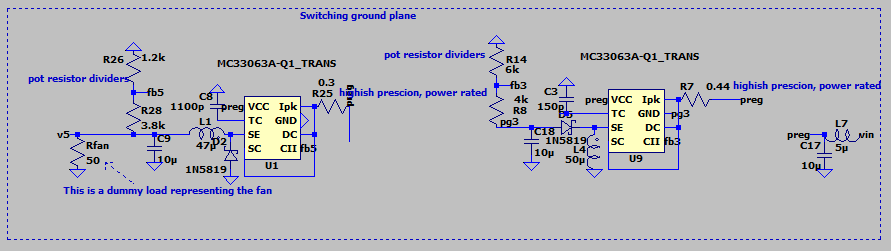
\includegraphics[width=0.8\textwidth]{chase2}
    \caption{Switching Section}
    \label{fig:chase2}
\end{figure}


\begin{figure}[H]
    \centering
    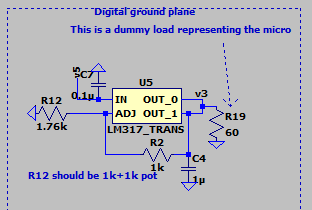
\includegraphics[width=0.8\textwidth]{chase3}
    \caption{Digital Section}
    \label{fig:chase3}
\end{figure}

The last two sections could be considered parts of a whole. These sections, the power and analog control, comprise of BJTs and op-amps mostly. The power section uses BJTs to control the 36 V from the Switched mode to the desired output voltage. To achieve this, op-amps take the feedback from the output of the power section and, along with control lines from the microchip, set the correct voltage to control the BJTs.\\

\begin{figure}[H]
    \centering
    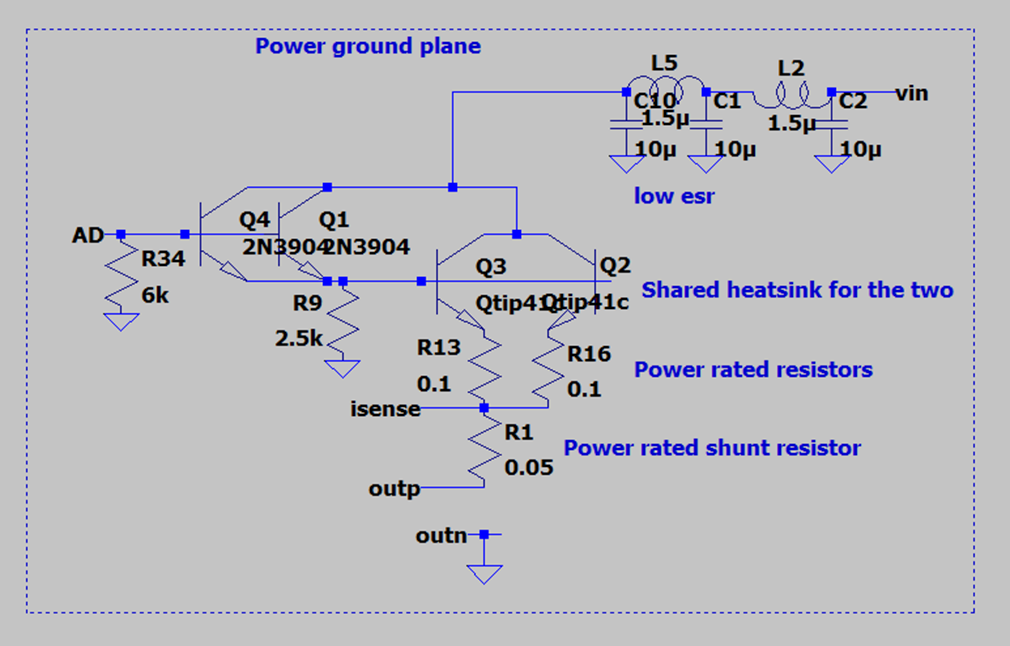
\includegraphics[width=0.8\textwidth]{chase4}
    \caption{Power Section}
    \label{fig:chase4}
\end{figure}

\begin{figure}[H]
    \centering
    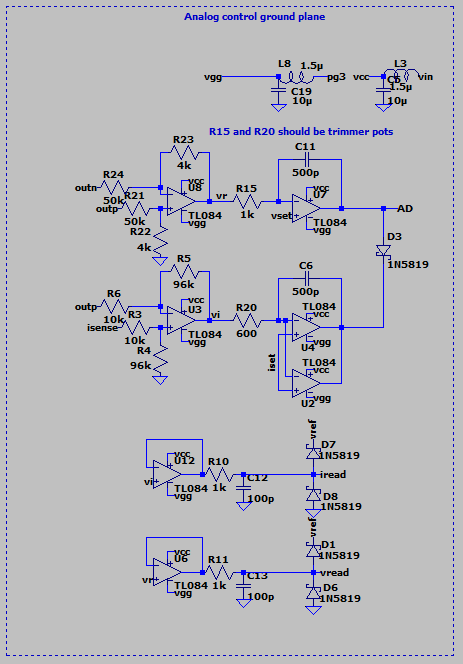
\includegraphics[width=0.6\textwidth]{chase5}
    \caption{Power Section}
    \label{fig:chase5}
\end{figure}

Throughout the linear stage, ceramic capacitors are preferred as they naturally have a low ESR and generally have a smaller footprint. Most resistors are of a general SMD type with a few notable differences. The resistors at the output on the power section need to be power rated which makes them much larger than a 0805 resistor. There are also several potentiometers used throughout the design which allow a greater control for fine tuning for the regulators and op-amps. Most other parts are standard and can be purchased in large quantities for a relatively cheap price.\\


\begin{figure}[H]
    \centering
    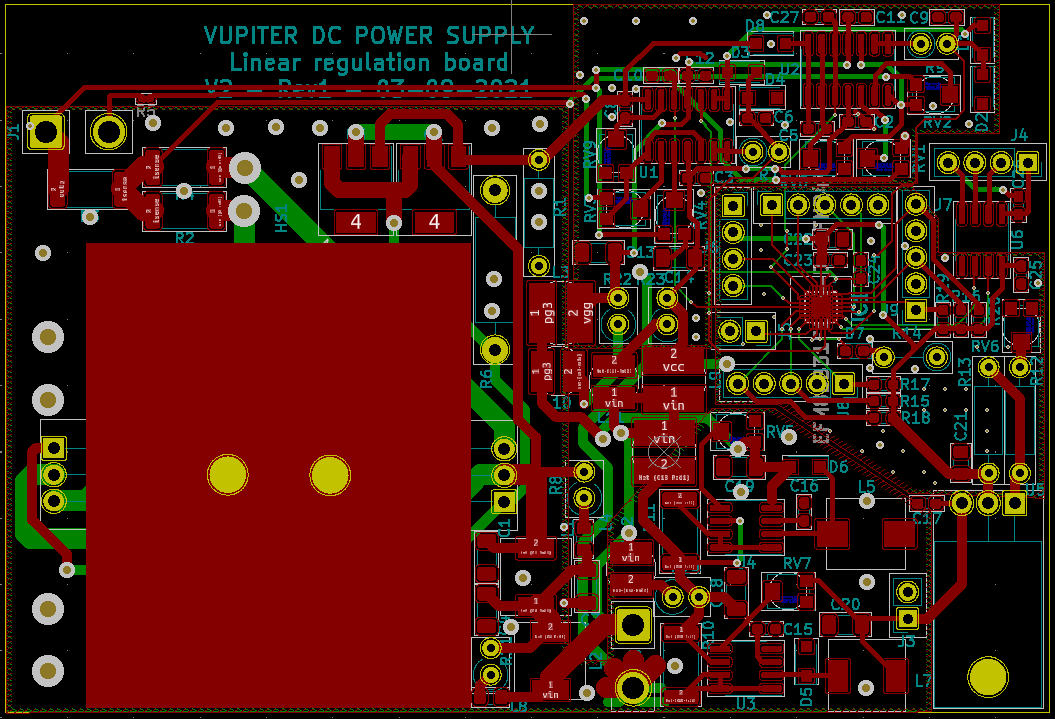
\includegraphics[width=0.8\textwidth]{chase6}
    \caption{Linear Board Design}
    \label{fig:chase6}
\end{figure}
\pagebreak
\section{AC/DC Topology Design - Alex Jones}
The original plan for the AC to DC stage design was a singular switch-mode converter per channel to supply voltage transformation and isolation. Ultimately this cannot work, as the linear stage’s need for a variable supply combined with potentially varied AC supply would put impossible duty cycles on the forward converter for any given transformer setup. For example, at the two extremes we need to support both 85 VAC to 36 VDC and 265 VAC to 6 VDC. The first of these is a ratio of 3:1 while the other is a ratio of 63:1. That level of versatility in a supply is simply impossible due to switching speeds and the need to reset the inductor.\\

This issue strongly indicates the need for an additional switch mode supply in the chain. This second supply would allow for each converter to have either a fixed input or a fixed output, instead of variable requirements on both. A common choice for this problem is an input power factor correction circuit. Firstly, PFC is required by IEC 61000-3-2 for all consumer devices. Secondly common PFC topologies increase the total voltage to an intermediary 400 VDC supply. This is useful as it decreases current stress and inductance requirements on the subsequent forward converter. \\

Thus, our final topology for the AC to DC converter stage is a boost power factor correction circuit followed by a forward converter. This addition kills two birds with one stone in that it is a pre-regulator, reducing complexity and stresses on the forward converter, and it helps the total device be standard compliant.  This topology is represented in Figure 1.

\begin{figure}[H]
    \centering
    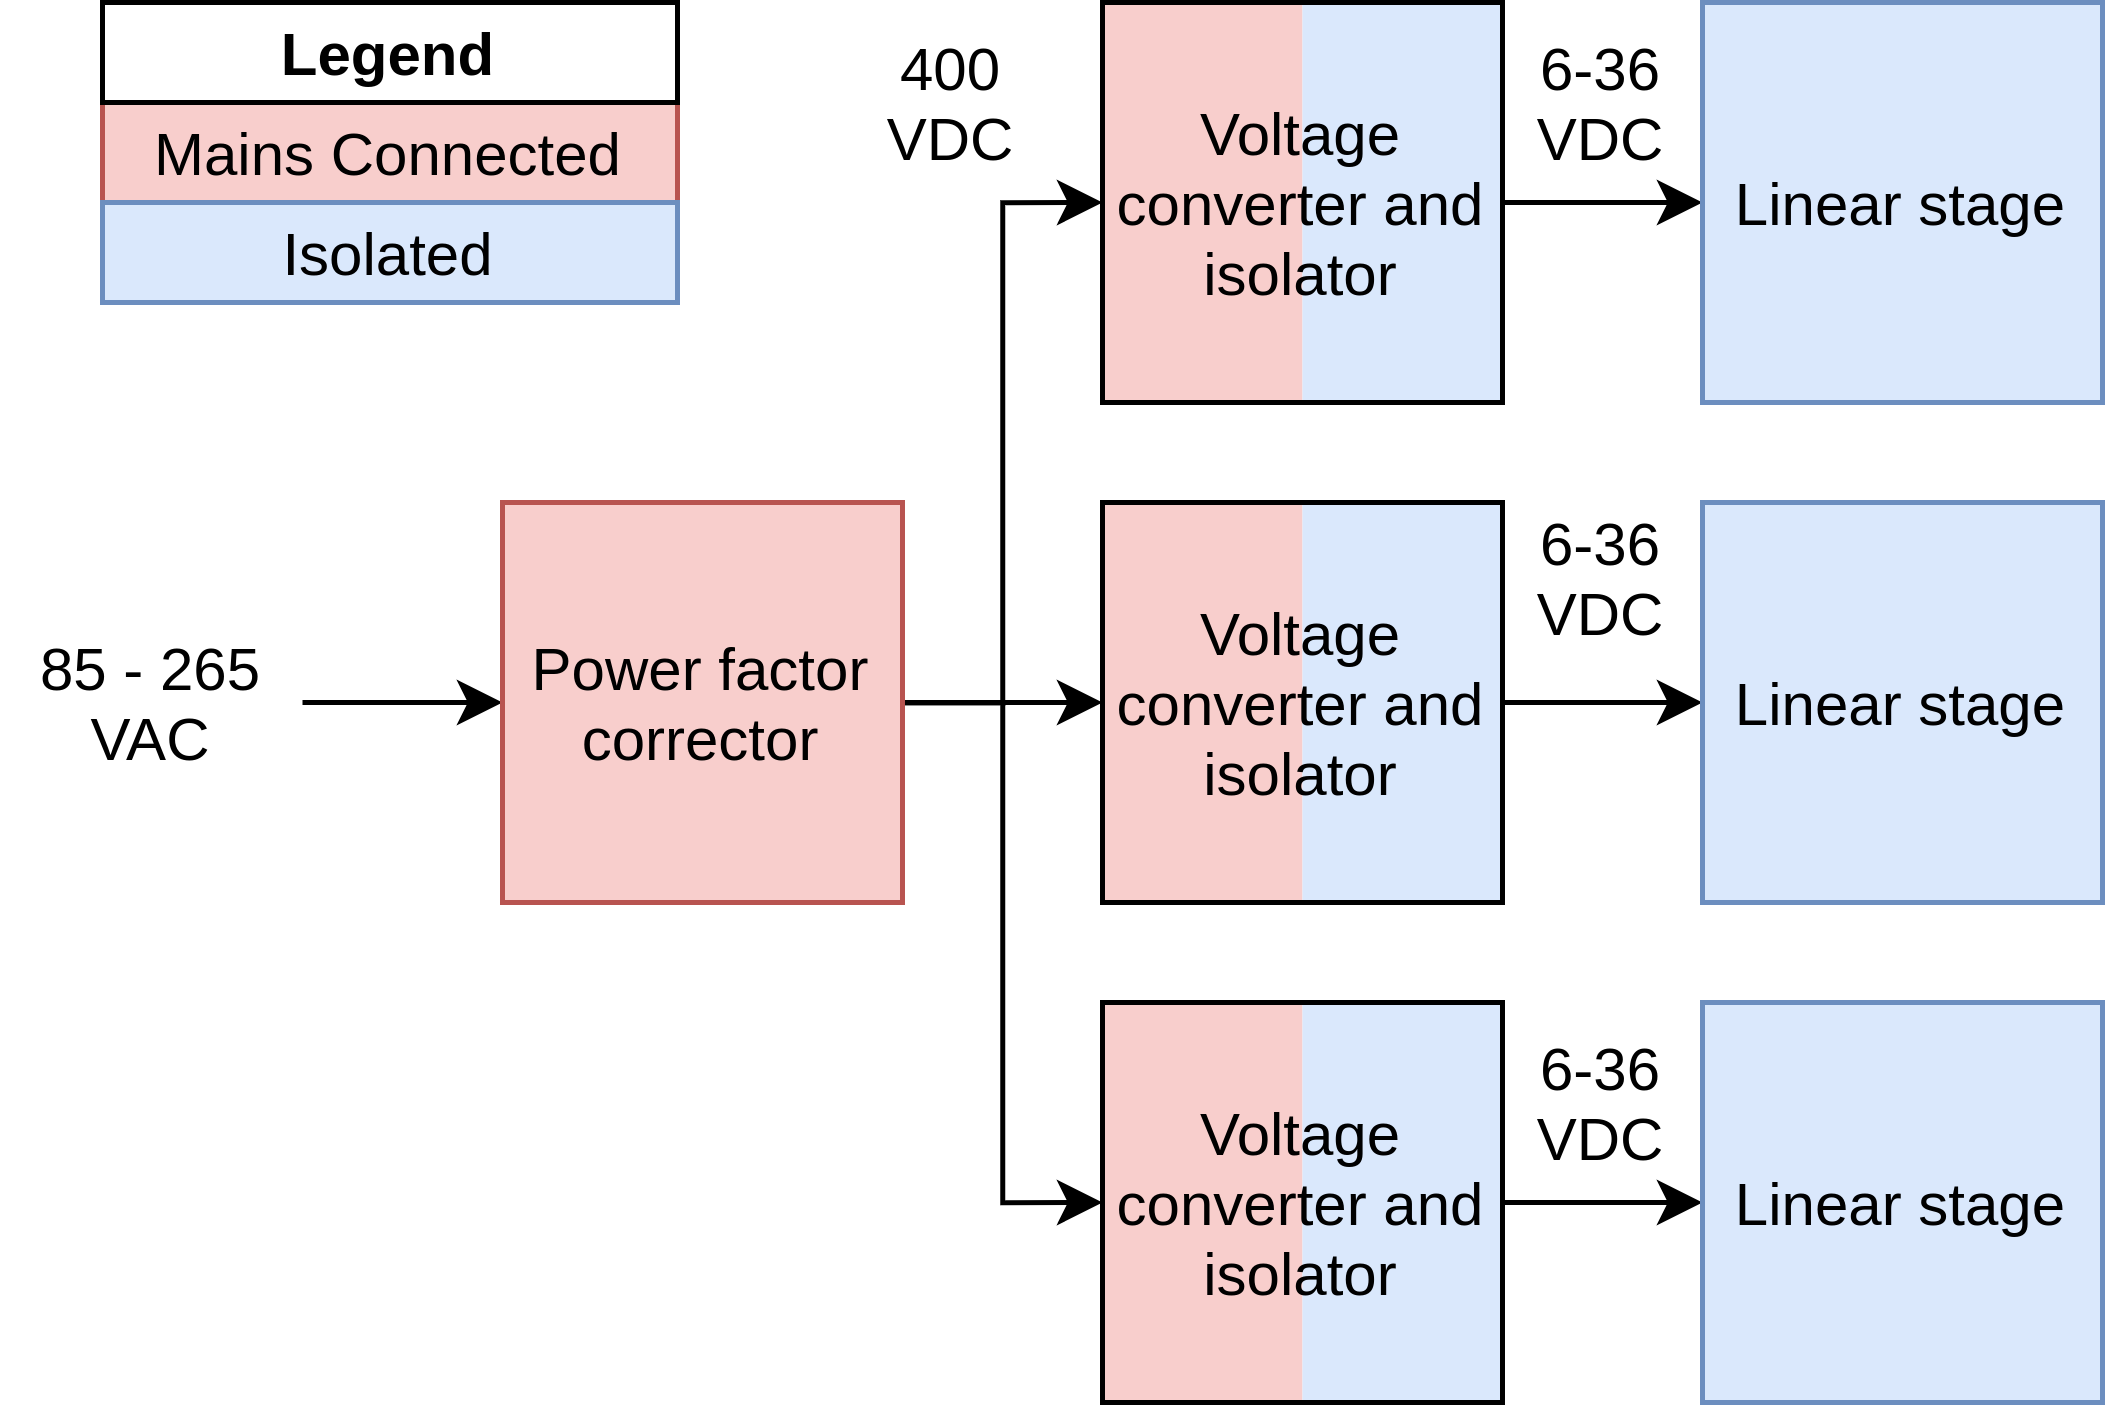
\includegraphics[width=0.8\textwidth]{acdctopo}
    \caption{AC to DC stage topology}
    \label{fig:acdctopo}
\end{figure}

\section{PFC stage  - Alex Jones}
\subsection{Requirements}
\begin{itemize}
\item 85-265 VAC input \begin{itemize}
    \item This is a widely accepted “universal” input range
\end{itemize}
\item 400 VDC output \begin{itemize}
    \item Common PFC designs rely on boost converters, requiring the intermediary design voltage to be higher than the maximum input voltage. Our 265 VAC input peaks at 370 volts, and this is increased to 400 volts nominally.
\end{itemize}
\item 600 watt total output \begin{itemize}
    \item Each channel can supply 150 watts, giving us a 450 watt total. 30 watts are added to each channel for the linear regulation. This leaves us at 540 watts. 600 watts was selected for some efficiency headroom and to prevent major voltage droops at full load.
\end{itemize}
\item 0.9 Power factor \begin{itemize}
    \item Not required in the US but the EU requires IEC 61000-3-2\cite{4} which wants power factor correction in all consumer devices. 
\end{itemize}
\end{itemize}


\subsection{Design}
PFC controller IC’s are available commercially. These frequently detail design equations for major components such as the primary inductor. Our selected controller is the BD7692FJ due to price and availability, as well as its thorough documentation allowing us to verify our design against known good equations. Its reference board is detailed thoroughly in \cite{1}. We selected a switching frequency of 500 kHz as this high frequency minimizes the size of inductors and filters needed, while not causing excessive switching losses in the cheaper range of diodes and mosfets. As the PFC resides before isolation, we opted to design a singular PFC to supply all 3 channels rather than 3 independent PFCs. This choice was dictated by the availability and cost of appropriately sized PFC controllers. \\

The schematic of this PFC unit is in \autoref{fig:PFC}. A number of values in this schematic are quite different from their ideal values in the name of BOM reduction, especially in the snubbers and filters where exact values are relatively unimportant. The passive components surrounding the mosfet gate are very similar to the gate circuitry implemented on the isolation stage, and they are there to ensure proper startup function and mosfet protection, which is critical in noisy inductive applications. Notably missing from \autoref{fig:PFC} is any form of EMI filter. This has yet to be designed, but the design of it will follow Mühlethaler et. al.\cite{8} as their paper details emi filter design specifically for PFC units. Right now the PFC would not be compliant with a number of standards, most notably IEC 61000-2-3 \cite{3} which regulates non-harmonic conduction back into mains.\\

One of the most critical components in any boost converter is the primary inductor. Due to the sinusoidal input and high desired output power this inductor must tolerate extremely high peak currents. For our design criterion in the worst case of an 85 volt input this peak is approximately 20 amps. This far exceeds typical commercial inductor’s saturation limit, at least in our price range. Thus we are required to wind our own inductor using ferrite cores. Erickson et. al.\cite{2} lays out a procedure for designing gapped inductors from commercially available cores. This procedure was followed to design the inductor used in these converters with cores purchased from digikey. The core will be wrapped with litz wire from ebay.\\

\begin{figure}[H]
    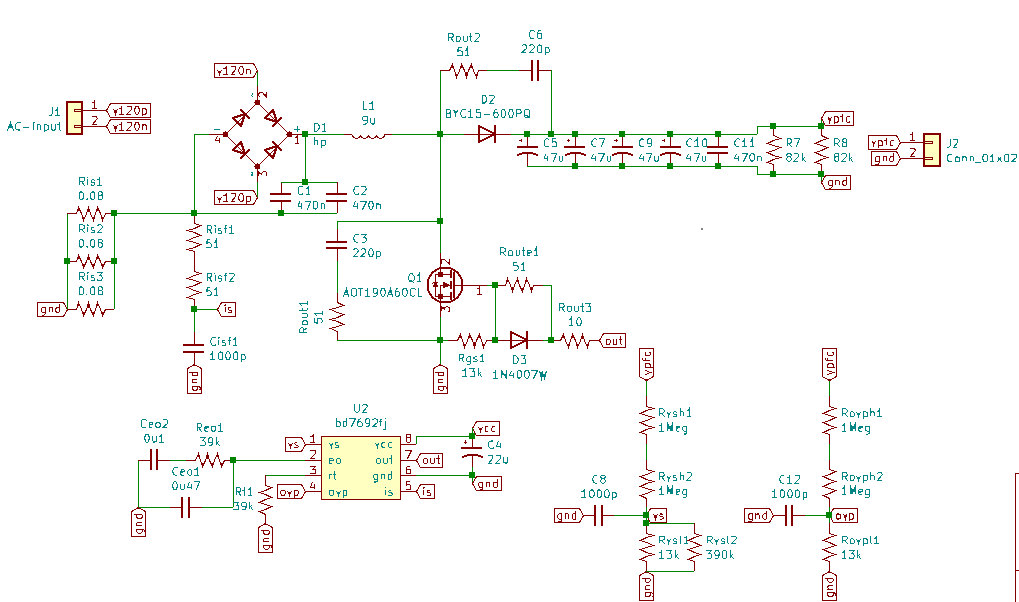
\includegraphics[width=\textwidth]{pfcschema}
    \caption{PFC converter schematic}
    \label{fig:PFC}
\end{figure}

The PFC controller IC requires a supply voltage and has no provisions to efficiently bootstrap from the high input voltage. With efficiency as a design goal, classic zener and resistor setups are unacceptable. Instead we opt for a small offline converter based around the AP3917B. This regulator can be seen in \autoref{fig:buck}. The AP3917B is specifically designed for these offline applications as not only does it tolerate the high voltages but it can also drive it’s internal switch at extremely low duty cycles, a key factor in such a large voltage transformation. The design of this converter is detailed thoroughly in a manufacturer application note in \cite{7}. With rough component values provided by those equations, exact component selection came down once again to BOM reduction, trying to utilize as many of the same parts as the PFC circuitry. This converter is tuned for 15 volts and is also exported off board to serve as a supply voltage for the control logic in the isolation stage, drastically improving their efficiency as well.\\

\begin{figure}[H]
    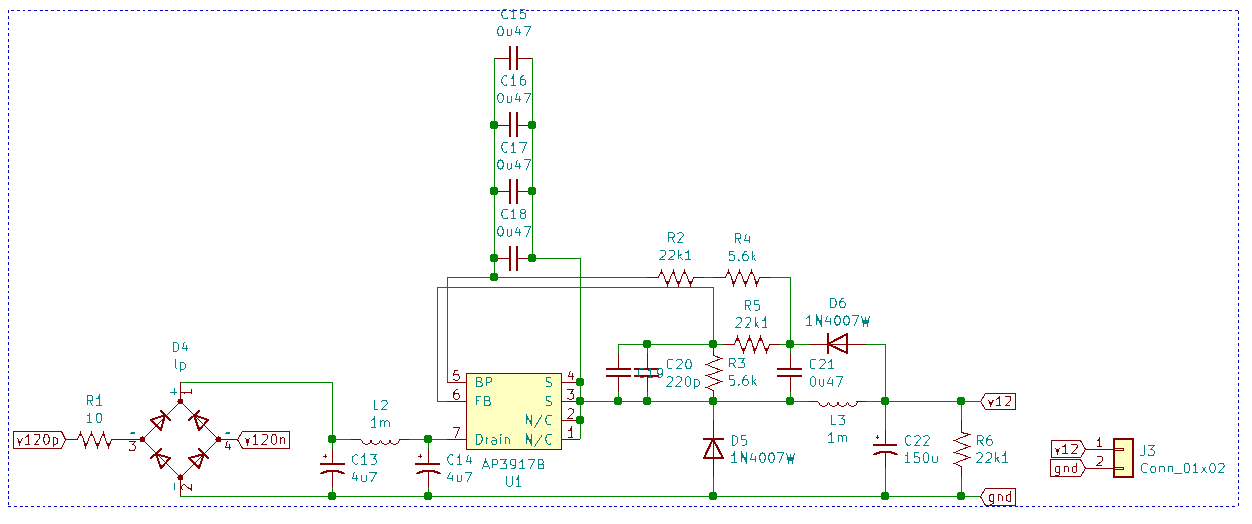
\includegraphics[width=\textwidth]{pfcbuck}
    \caption{15 volt offline buck converter design}
    \label{fig:buck}
\end{figure}
    
These two converters, the boost PFC and the offline buck go on one board, whose layout can be seen in \autoref{fig:pfclayout}. The buck converter is located along the bottom edge of the board while the PFC module occupies the rest of the board. The EMI filter will either be placed in the currently unoccupied top left of the board or on a separate board. The price for this board including the pcb itself, all the components, and the litz wire needed to wind the inductor comes out to 18 dollars.\\
\begin{figure}[H]
    \centering
        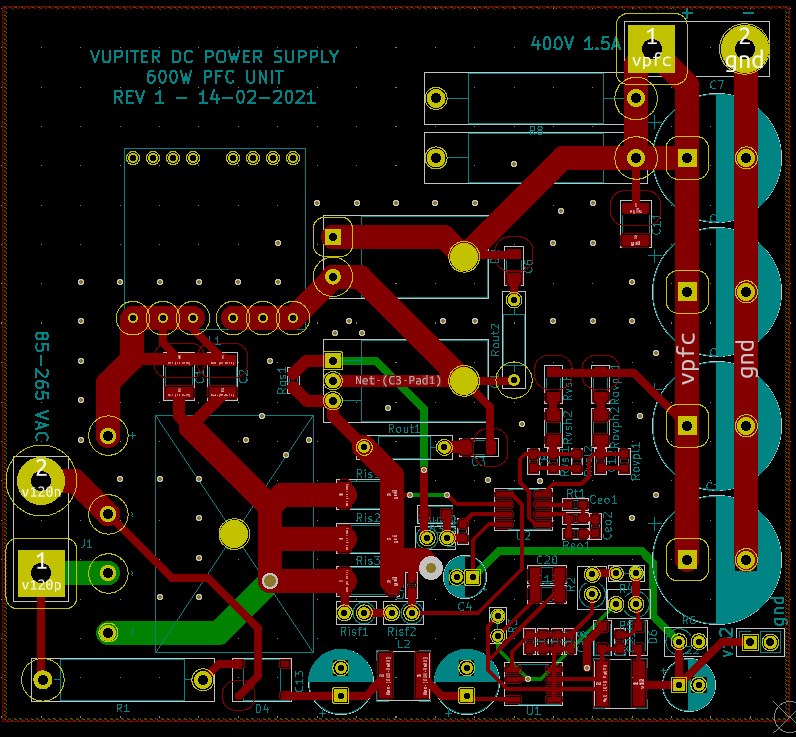
\includegraphics[width=0.75\textwidth]{pfclayout}
        \caption{PFC board layout}
        \label{fig:pfclayout}
    \centering
\end{figure}

\section{Isolation stage  - Alex Jones}
\subsection{Requirements}
\begin{itemize}
\item 400 VDC input \begin{itemize}
    \item This is coming from the PFC module, nominally 400 but we are designing for 380-420 actually
\end{itemize}
\item 36-6 VDC output \begin{itemize}
    \item The linear stage needs this variable output for efficiency and heat purposes. The board needs to automatically adjust to an input signal plus 6 volts. This 6 volts is the headroom the linear stage needs to both increase and decrease its output. This automatic adjustment should be highly bandwidth limited to prevent oscillations
\end{itemize}
\item 5.5 amp output \begin{itemize}
    \item Each channel can only supply 5 amps at any given voltage, and the additional 0.5 amps is allocated to supply all the auxiliary functions.

\end{itemize}
\item Full isolation \begin{itemize}
    \item This is important for both safety and functionality. The most notable standard requiring this isolation is IEC 62368 \cite{5}. From a functionality point of view, we want isolation so that we can use multiple channels in series for greater voltage ranges or as a bipolar supply.
\end{itemize}
\end{itemize}
\subsection{Design} 
For this design we chose a two-switch forward converter, which has a number of advantages for this type of application. Firstly, being a buck derived converter, the output inductor has a constant waveform through it thus handling the majority of demand, reducing the need for costly and bulky capacitors. Secondly, the transformer design is simplified by the lack of any tertiary or reset windings such as in flyback converters. Third and possibly most critical, forward converters, unlike their resonant counterparts, can drastically vary their output range whereas modern LLC converters would struggle to deviate from the designed voltage.  The pros and cons of various topologies are discussed more in depth in Erickson et. al.\cite{2}.\\

Our converter is based around the NCP1252, chosen for its low cost and thorough documentation. As before, the manufacturer provides a document detailing the design of a reference board in \cite{9}. Our design has major deviations from this simple example, first and foremost in the isolated feedback section. This feedback network can be seen in \autoref{fig:forwardback}. It has been complicated substantially from traditional designs due to the wide range of outputs this supply most allow. The optocoupler is powered from a regulated supply to ensure that the gain of the control loop is not impacted by the current output level. The feedback itself is managed by a differential amplifier to create the rather unique feedback plus volts effect.

\begin{figure}[H]
    \centering
    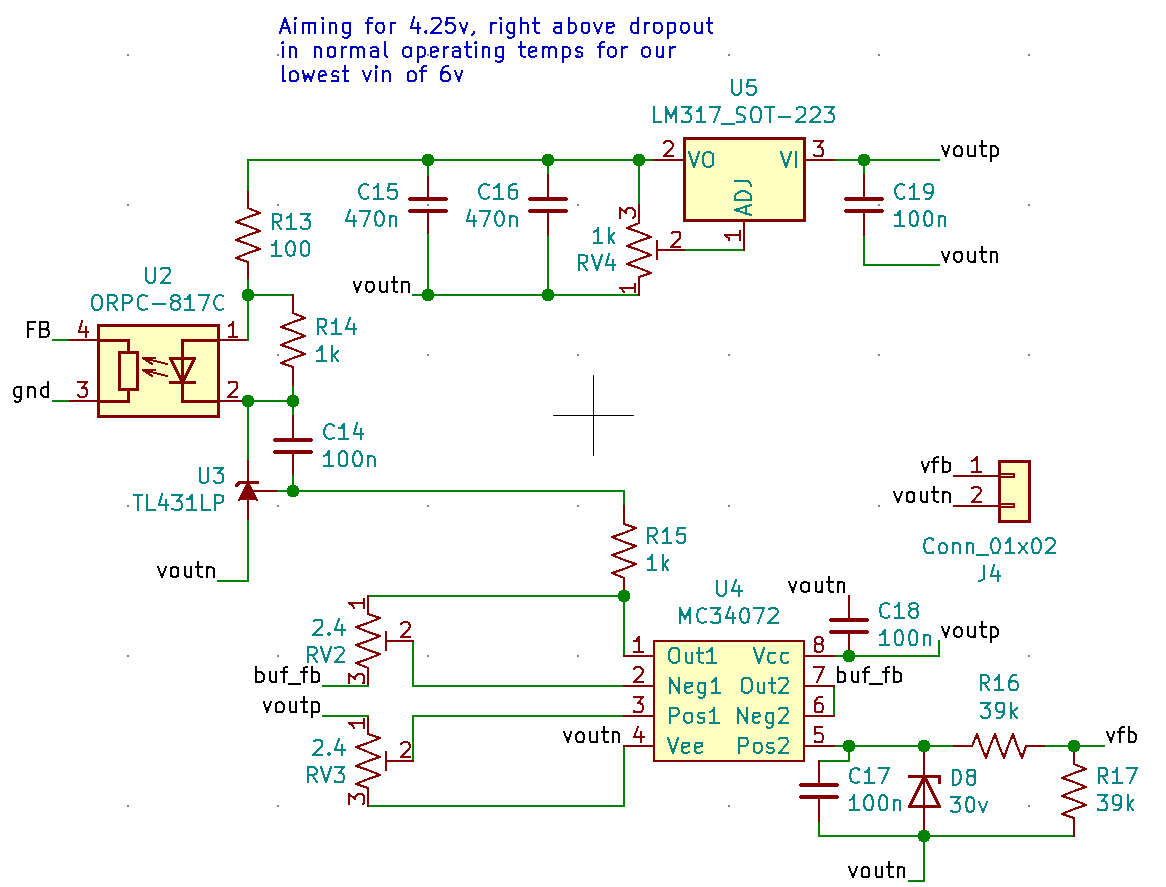
\includegraphics[width=0.5\textwidth]{forwardfeedback}
    \caption{Isolated feedback drive}
    \label{fig:forwardback}
\end{figure}

The bulk of the converter is in \autoref{fig:forwarddrive}. The gate driving is accomplished by a bootstrap gate driver IC This driver generates the voltages needed for high-side driving of the N-channel mosfets used. This is both a cost and size reduction when compared with using a gate driver transformer. About 25\% of the components in the feedback section and this gate driver section are shared with the PFC board as a BOM reduction method.

\begin{figure}[H]
    \centering
    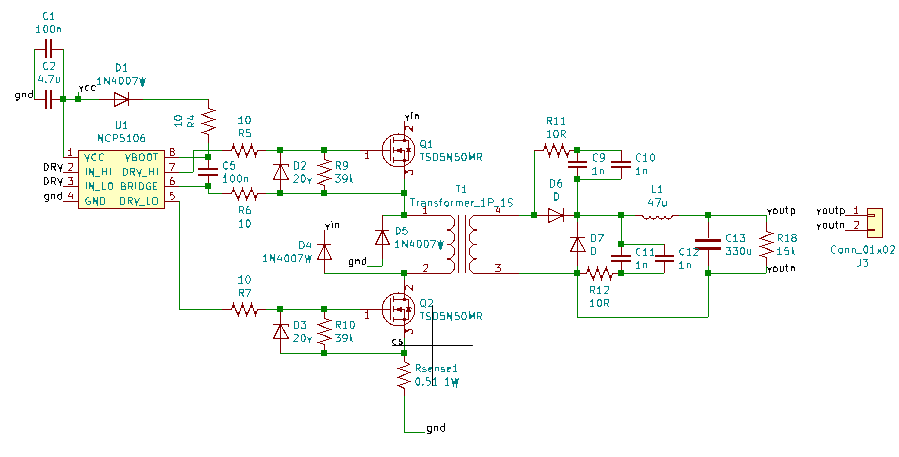
\includegraphics[width=0.75\textwidth]{forwarddrive}
    \caption{Forward converter design}
    \label{fig:forwarddrive}
\end{figure}

The transformer used in \autoref{fig:forwarddrive} is custom made and wound with litz wire, the same as the PFC inductor. Once again, Erickson et. al.’s\cite{2} procedure was used to design the transformer from commercially available cores. In addition to the insulation on the wires, polyimide tape will be added between the primary and secondary windings to add redundant isolation, in accordance with IEC 62368\cite{5}.\\

These two sections reside on one board with a large gap in the ground plane for isolation. This layout is in \autoref{fig:forwardlay}. The gap between underneath the transformer and optocoupler exceeds IPC2221A\cite{6} creepage and clearance specifications by a factor of 2. The total BOM cost including the wire to wrap the transformer totals 6 dollars, or 18 dollars for the entire supply as there are three of this board.
\begin{figure}[H]
    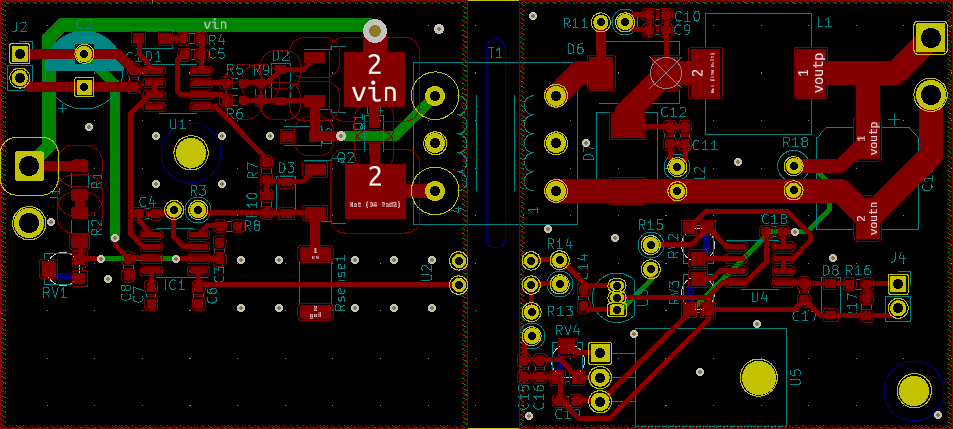
\includegraphics[width=\textwidth]{forwardlayout}
    \caption{Forward converter design}
    \label{fig:forwardlay}
\end{figure}

\section{Computer Interface - Rice Shelley}
The Vupiter DC power supply will have a computer interface supported by USB 2.0 and SCPI (Standard Commands for Programmable Instruments). The SCPI protocol will exist on top of the USB layer. The USB spec will be met with an FTDI chip that converts USB 2.0 to UART. The SCPI protocol interpreter is embedded into one of the power supply’s microcontrollers. The relatively simple SCPI protocol allows easy development of desktop software to control the power supply. The power supply will implement the DCPSUPPLY SCPI\cite{10} base class to ensure basic compatibility with other SCPI power supply control software. The DCPSUPPLY SCPI standard can be found in Reference 1. An example of power supply control using SCPI is shown below. \\
\\
*RST\\
INSTrument:NSELect 1\\
SOURce:VOLTage:LEVel:IMMediate:AMPLitude 12V\\
OUTPut:STATe ON\\
\\\\
This SCPI command sequence would reset the power supply, select channel one, set the voltage to 12 volts, and then enable the output. 


\section{User Interface - Al Spies}
User interface allows user to control device from front panel while viewing voltage and current readings from each channel of the power supply. Adjustments are made with encoders and variables can be viewed on 128 x 68 OLED display. User interface control is done with EFM8 board. User has option to control system with computer through communication to EFM8 board using UART protocol that are built into the design. Each channel of the power supply will have its own EFM8 board, encoders, and display. EFM8 board coding will be designed using Simplicity Studio software.\\

\noindent \textbf{Functions of EFM8}:
\begin{itemize}
    \item Receive encoder signals \begin{itemize}
        \item Voltage encoder  \begin{itemize}
            \item Channel A
            \item Channel B
            \item Optional Button
        \end{itemize}
        \item Current encoder  \begin{itemize}
            \item Channel A
            \item Channel B
            \item Optional Button
        \end{itemize}
    \end{itemize}
    \item Receive analog signal from linear stage through onchip ADC \begin{itemize}
        \item Voltage
        \item Current
    \end{itemize}
    \item Send analog control signal to linear stage through onchip DAC \begin{itemize}
        \item Voltage
        \item Current
    \end{itemize}
    \item Send $I^2C$ control signals to OLED Display
    \item Communicate with UART computer interface board
\end{itemize}
\pagebreak
\section{Case Construction - Al Spies}
	Case used to house components of system will be made out of two metal plates that are bent to dimensions 300mm x 300mm x 65mm when assembled together with a 3D printed front panel. Vent holes drilled manually in sides for forced air flow to keep system within normal operating temperatures. Design is intended to be easily assembled so anyone can build with common tools in a household. Standards that apply to the device construction related to safety concerns are CFR §1500.49\cite{11}, IEC 62368\cite{5}, IEC 60950-1\cite{13}, and NFPA 70\cite{12}.

\noindent


All files, including this proposal are hosted on our github:\\
\url{https://github.com/ams0187/Vupiter}
\pagebreak
\raggedright
\begin{thebibliography}{9}
    \bibitem{1} 
    “Boundary Current Mode Method 200 W 400 V BD7692FJ Reference Board ,” 2019. [Online]. Available: \url{https://fscdn.rohm.com/en/products/databook/applinote/ic/power/acdc_converter/bd7692fj-evk-001_ug-e.pdf}

    \bibitem{2} 
    R. W. Erickson and Maksimovic Dragan, Fundamentals of power electronics. New York, New York: Springer Science + Business Media, 2012.

    \bibitem{3}
    IEC, “Description of the environment - Radiated and non-network-frequency-related conducted phenomena,” IEC Webstore, 1992. [Online]. Available: 
    \url{https://webstore.iec.ch/publication/4134}

    \bibitem{4}
    IEC, “Electromagnetic compatibility (EMC) - Part 3-2: Limits - Limits for harmonic current emissions (equipment input current 16 A per phase),” IEC Webstore, 2018. [Online]. Available:
    \url{https://webstore.iec.ch/publication/28164}

    \bibitem{5}
    IEC, “Audio/video, information and communication technology equipment - Part 1: Safety requirements,” IEC Webstore, 2018. [Online]. Available: 
    \url{https://webstore.iec.ch/publication/27412}

    \bibitem{6}
    IEC, “Generic Standard on Printed Board Design” IPC, 2003. [Online]. Available: \url{https://www.ipc.org/TOC/IPC-2221A.pdf}

    \bibitem{7}
    “1.44W AP3917B EV1 Evaluation Board User’s Guide,” Diodes Incorporated, 20-Feb-2020. [Online]. Available: \url{https://www.diodes.com/assets/Evaluation-Boards/1.44W-AP3917B-Single-Output-12V-120mA-EV1-User-Guide-Rev-1.1-Eval-Board-User-Guide.pdf}

    \bibitem{8}
    J. Mühlethaler et. al., “Optimal design of EMI filters for single-phase boost PFC circuits,” IEEE Xplore, 2012. [Online]. Available: 
    \url{https://ieeexplore.ieee.org/document/6388754}
    \bibitem{9}
    “AND8373/D - 2 Switch-Forward Current Mode Converter,” 2010. [Online]. Available: \url{https://www.onsemi.com/pub/collateral/and8373-d.pdf}

    \bibitem{10}
    “Standard Commands for Programmable Instruments (SCPI) - Volume 1: Syntax and Style,” IVI Foundation, 1999. [Online]. Available: \url{https://www.ivifoundation.org/docs/scpi-99.pdf}

    \bibitem{11}
    “16 CFR § 1500.49 - Technical requirements for determining a sharp metal or glass edge in toys and other articles intended for use by children under 8 years of age.,” Legal Information Institute. [Online]. Available: \url{https://www.law.cornell.edu/cfr/text/16/1500.49}
    
    \bibitem{12}
    “NFPA 70,” NFPA 70®: National Electrical Code®. [Online]. Available: \url{https://www.nfpa.org/codes-and-standards/all-codes-and-standards/list-of-codes-and-standards/detail?code=70.} 
    
    \bibitem{13}
    IEC, “Electromagnetic compatibility (EMC) - Part 3-2: Limits - Limits for harmonic current emissions (equipment input current 16 A per phase),” IEC Webstore, 2005. [Online]. Available:
    \url{https://webstore.iec.ch/publication/4024}
\end{thebibliography}
\end{document}